\chapter{Open Source MANO}
\label{ch:osm}
\section{Configuration requirements needed to run Open Source MANO (OSM) Release FOUR is a single server or VM:}
		\begin{itemize}
	\item MINIMUM: 2 CPUs, 4 GB RAM, 20GB disk and a single interface with Internet access
	\item RECOMMENDED: 2 CPUs, 8 GB RAM, 40GB disk and a single interface with Internet access
	\item Ubuntu16.04 (64-bit variant required) as base image 
	(\hyperlink{name}{http://releases.ubuntu.com/16.04/})
		\end{itemize}
\section{Open Source Mano Installation}
\subsection{Steps for Installation:}
\begin{itemize}
	\item Downloading latest version of OSM
	\begin{lstlisting} 
	wget https://osm-download.etsi.org/ftp/osm-4.0-four/install_osm.sh
	\end{lstlisting}
	
	\item Installing OSM
	\begin{lstlisting} 
	chmod +x install_osm.sh
	$ ./install_osm.sh 2>&1 | tee osm_install_log.txt
\end{lstlisting}
\end{itemize}
\subsection{verifying installation from the OSM GUI:}
\begin{itemize}
\item Accessing GUI:
\begin{lstlisting} 
Access http://1.2.3.4, replacing 1.2.3.4 with the IP address of your host.
Login using Userid : admin , password : admin
\end{lstlisting}

\begin{figure} [H]
	\centering
	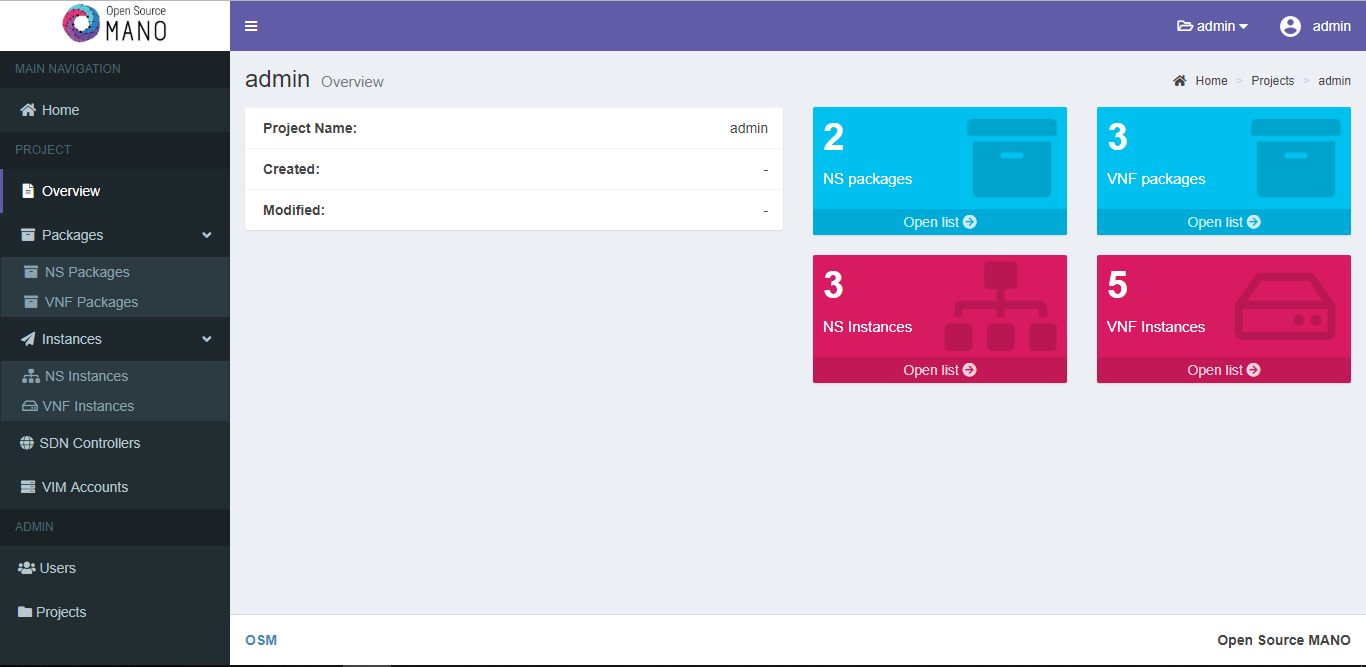
\includegraphics[width=0.5\linewidth]{figures/Sh1}
	\caption{OSM GUI}
\end{figure}

\item Verify 10 docker containers were created:
\begin{lstlisting} 
docker stack ps osm |grep -i running
docker service ls
\end{lstlisting}
\end{itemize}
\section{VIM Installation}
\subsection{Steps to install openstack using devstack are as follows:}
\begin{itemize}
\item Create a user “stack”
\begin{lstlisting}
sudo useradd -s /bin/bash -d /opt/stack -m stack
echo "stack ALL=(ALL) NOPASSWD: ALL" | sudo tee /etc/sudoers.d/stack
sudo su -stack
\end{lstlisting}
\item Clone the devstack repository
\begin{lstlisting}
git clone https://git.openstack.org/openstack-dev/devstack
cd devstack
\end{lstlisting}
\item Create and configure the local.conf file
\begin{lstlisting}
[[local|localrc]]
ADMIN_PASSWORD=password
DATABASE_PASSWORD=$ADMIN_PASSWORD
RABBIT_PASSWORD=$ADMIN_PASSWORD
SERVICE_PASSWORD=$ADMIN_PASSWORD
\end{lstlisting}
\item Execute the command
\begin{lstlisting}
./stack.sh
\end{lstlisting}
\item After installation check and verify from openstack horizon GUI:
\begin{lstlisting}
Access http://1.2.3.4, replacing 1.2.3.4 with the IP address of your host.
Login using Userid : admin , password : admin
\end{lstlisting}
\begin{figure} [H]
	\centering
	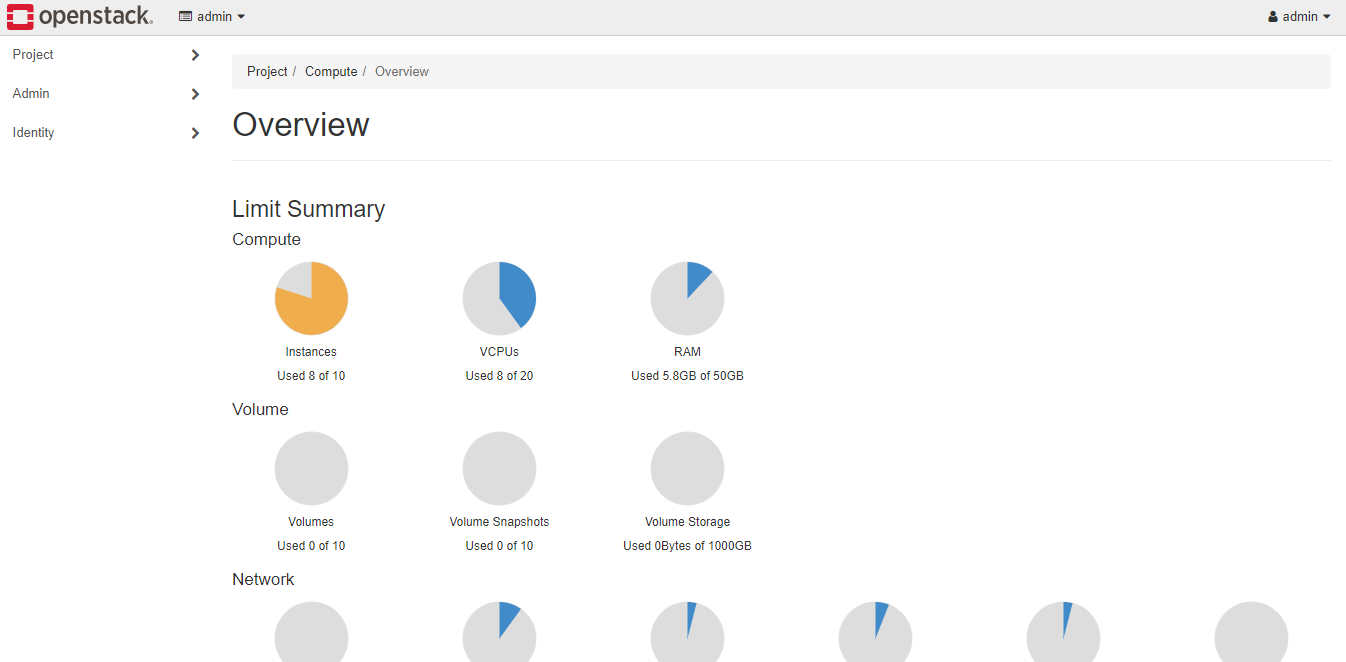
\includegraphics[width=0.5\linewidth]{figures/sh2}
	\caption{Open Stack Dashboard}
\end{figure}
\end{itemize}
\section{Configure openstack for OSM}
\begin{itemize}
\item Guarantee that Openstack API endpoints are reachable from OSM (particularly from RO container):
\begin{lstlisting}
Login to openstack api access from the horizon gui.
Click on DOWNLOAD OPENSTACK RC FILE (api version 3).
Copy the OS_AUTH_URL variable value.
Paste in the browser or do a curl from the VM where OSM is installed to check its reachability. 
\end{lstlisting}
\item Create a management network, with DHCP enabled, reachable from OSM (particularly from VCA container)
\begin{lstlisting}
Login to openstack horizon gui.
Go to admin-> create network.
Give the project name as your project ( default:admin)
Give a network name -> mgmt.
Give a network subnet name and network address (10.208.1.0/24). 
Keep the Network Address source as 'ENTER NETWORK ADDRESS MANUALLY'.
Keep Gateway IP blank.
In Allocation Pools, give the IPs:  start=10.208.0.2,end=10.208.0.254.
Leave DNS Name servers and Host Routes blank and click create.
\end{lstlisting}
\begin{figure}[H]
	\centering
	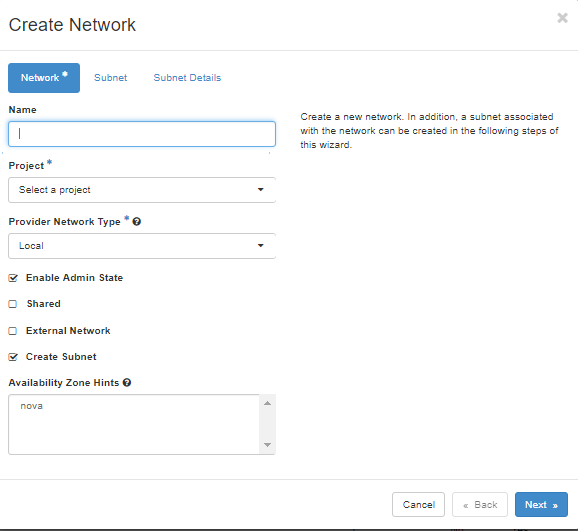
\includegraphics[width=0.5\linewidth]{figures/sh11}
	\caption{Creating a Network in Openstack}
\end{figure}
\item creating a valid tenant/user
\begin{lstlisting}
Login to openstack horizon gui.
Go to identity-> create user.
Give the project name as your project ( default:admin)
Give a user name -> tenant.
Give the role also as admin and click create.
\end{lstlisting}
\begin{figure} [H]
	\centering
	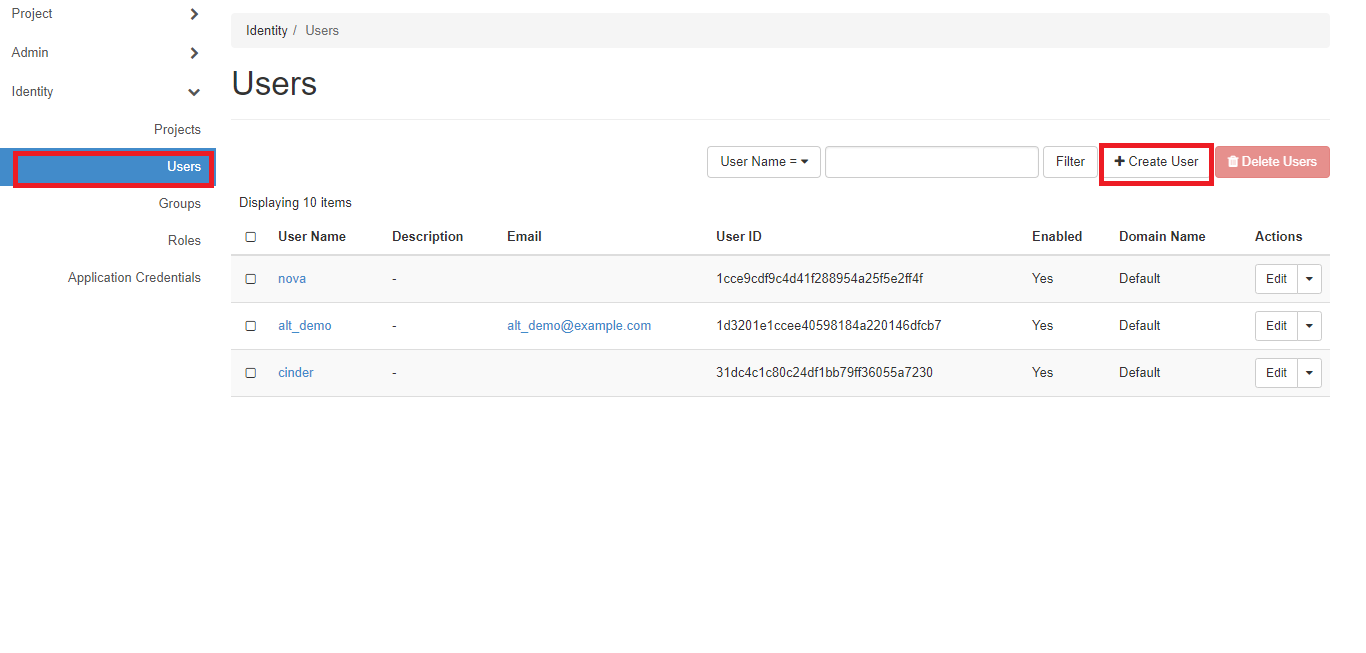
\includegraphics[width=0.5\linewidth]{figures/sh9}
	\caption{creating a valid tenant/user in openstack}
		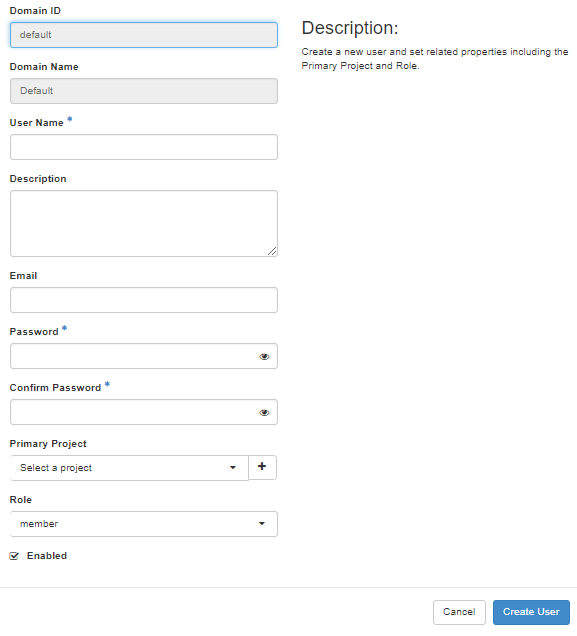
\includegraphics[width=0.5\linewidth]{figures/sh10}
	\caption{creating a valid tenant/user in openstack}
\end{figure}

\item Uploading VM image(s) to the VIM(s)
\begin{lstlisting}
Download the image from the following link: (\hyperlink{name}{http://download.cirros-cloud.net/0.3.4/cirros-0.3.4-x86_64-disk.img})
Login to openstack horizon gui.
Go to admin -> Compute -> Images and click on create image.
Give the image name 'cirros034'
Upload the downloaded image file in step 1.
Choose the image format as QCOW2 : QEMU Emulator
Click on create image.
\end{lstlisting}
\begin{figure} [H]
	\centering
	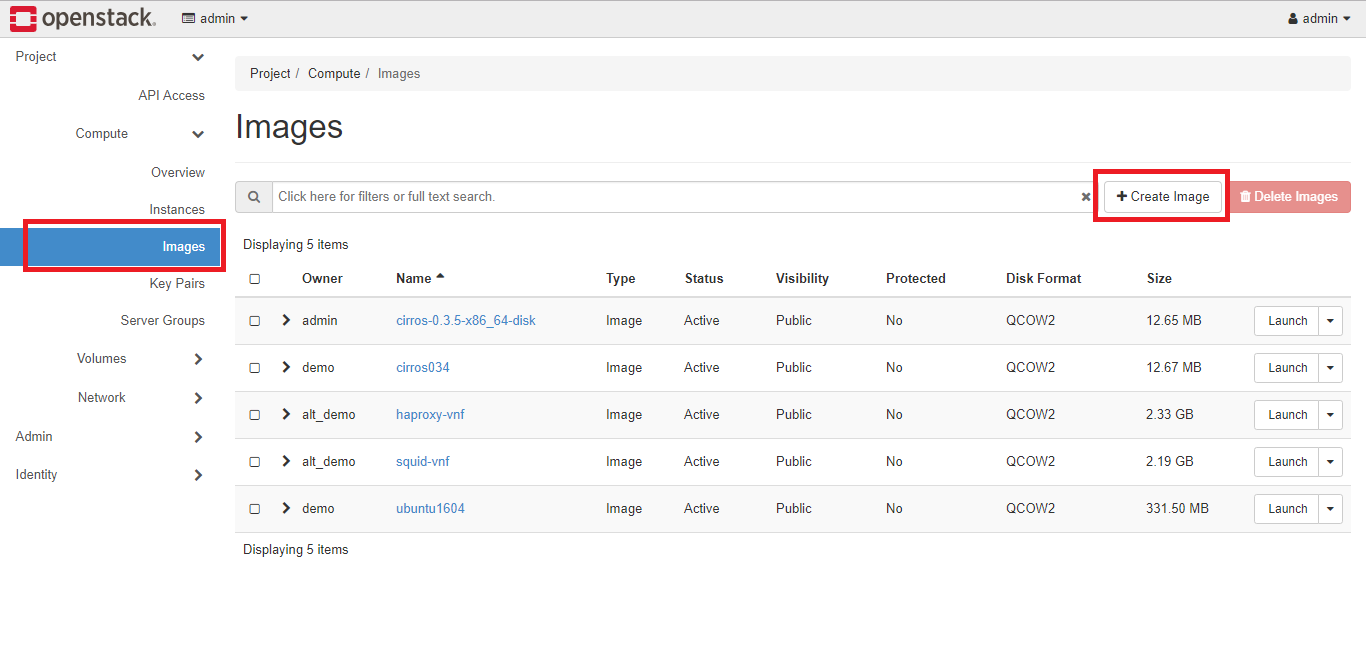
\includegraphics[width=0.5\linewidth]{figures/sh8}
	\caption{Uploading VM image to VIM in openstack}
\end{figure}
\item Adding VIMs to OSM
\begin{lstlisting}
Login to OSM and click on VIM Accounts.
Click on new VIM.
Give a name to your VIM instance and choose openstack from the type dropdown.Give the VIM URL as the OS\_AUTH\_URL variable value in openstack's rc file.
Enter the VIM userid and password as the login userid and password for openstack horizon gui.
Give the tenant name as admin/tenant.
Click on create.
\end{lstlisting}
\begin{figure} [H]
	\centering
	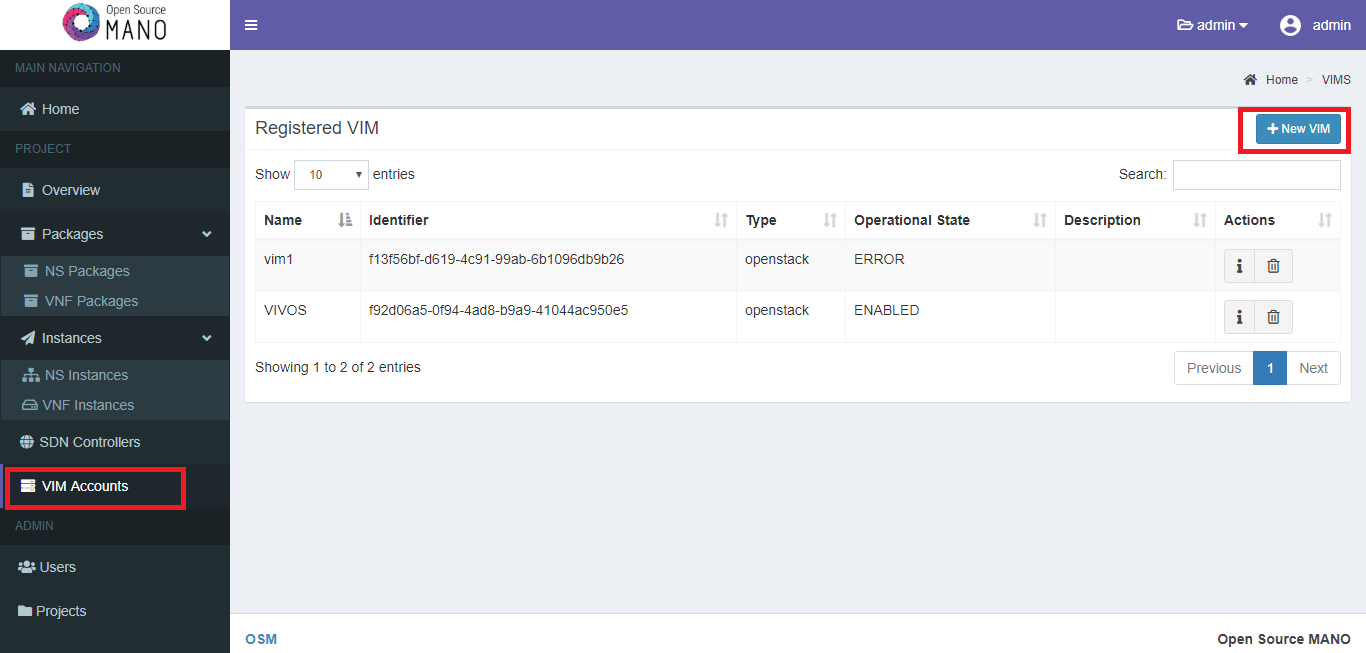
\includegraphics[width=0.5\linewidth]{figures/sh6}
	\caption{Adding VIMs to OSM}
	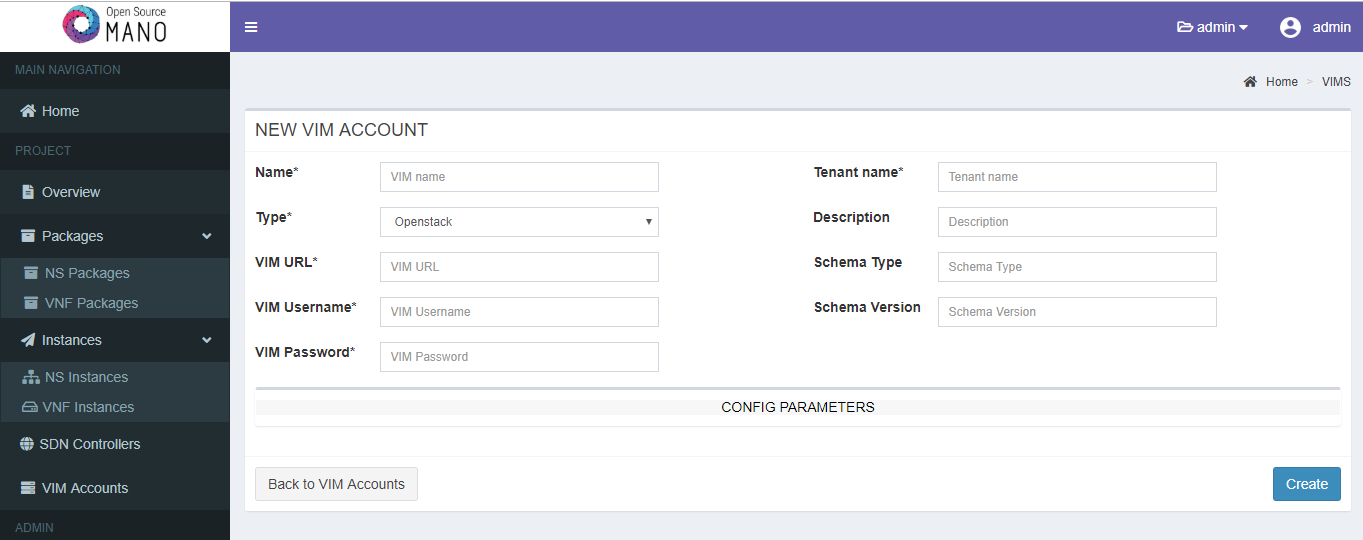
\includegraphics[width=0.5\linewidth]{figures/sh7}
	\caption{Adding VIMs to OSM}
\end{figure}
\end{itemize}
\newpage
\section{Deploying Network Service}
First download the required VNF and NS packages from this URL: \hyperlink{name}{(https://osm-download.etsi.org/ftp/osm-3.0-three/examples/cirros\_2vnf\_ns/)}
\begin{itemize}
\item On-boarding a VNFD
\begin{lstlisting}
From the UI , Go to Projects --> Admin --> VNF Packages (Open List)
Click on the Onboard VNFD button
Drag and drop the VNF package file cirros_vnf.tar.gz in the importing area.
\end{lstlisting}
\begin{figure} [H]
	\centering
	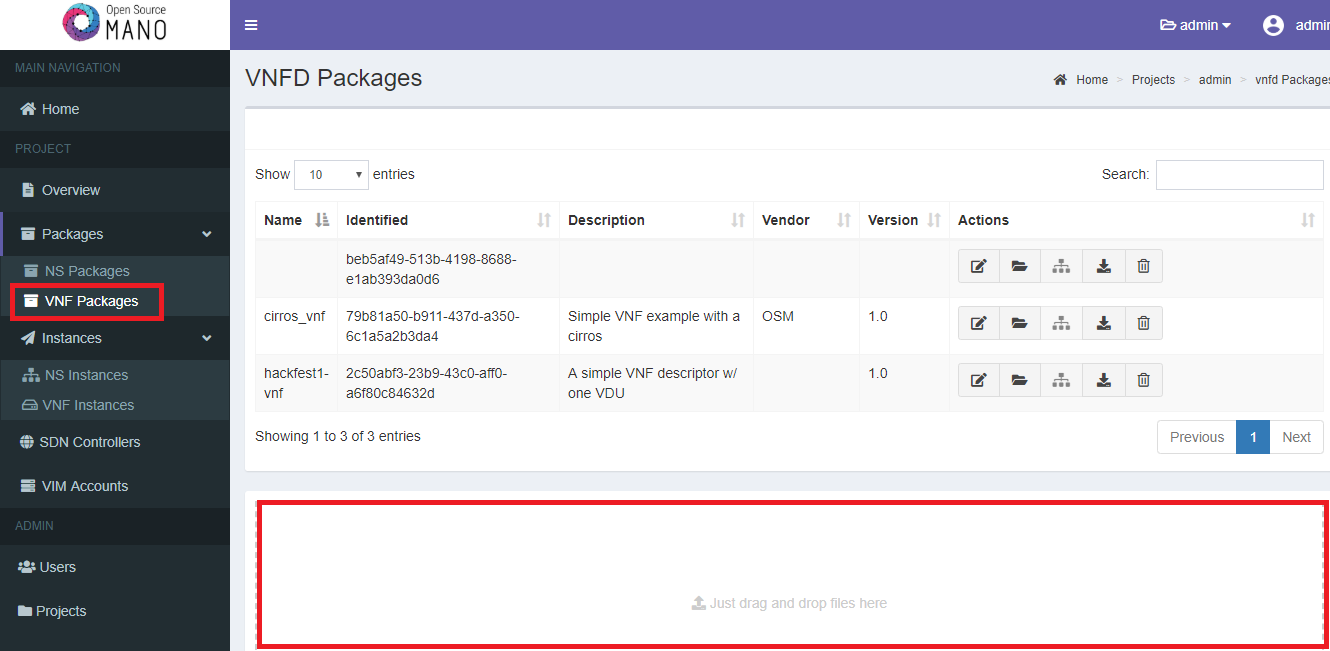
\includegraphics[width=0.5\linewidth]{figures/sh4}
	\caption{On-boarding of VNFD in OSM}
\end{figure}

\item Onboarding a NS
\begin{lstlisting}
From the UI, Go to Projects --> Admin --> NS Packages (Open List)
Click on the Onboard NSD button
Drag and drop the NS package file cirros_2vnf_ns.tar.gz in the importing area.
\end{lstlisting}
\begin{figure} [H]
	\centering
	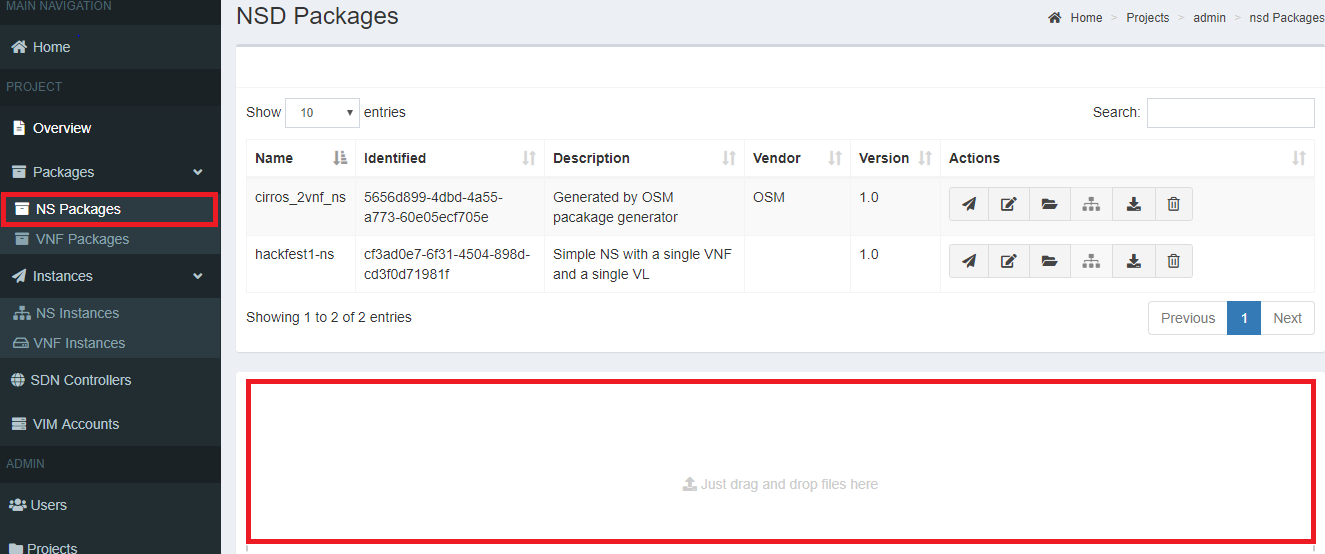
\includegraphics[width=0.5\linewidth]{figures/sh3}
	\caption{On-boarding of NS in OSM}
\end{figure}


\item Instantiating the NS
\begin{lstlisting}
From the UI, Go to Projects --> Admin --> NS Packages (Open List)
Next the NS descriptor to be instantiated, click on Launch
Fill the form, adding at least a name and selecting the VIM
\end{lstlisting}
\begin{figure} [H]
	\centering
	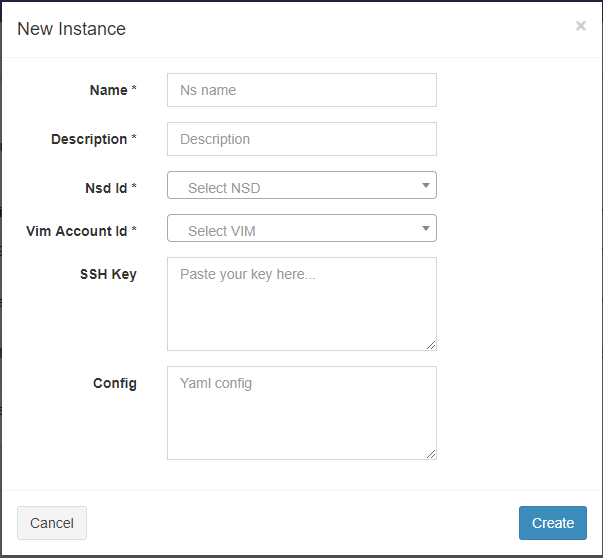
\includegraphics[width=0.5\linewidth]{figures/sh5}
	\caption{Initiating of NS in OSM}
\end{figure}
\end{itemize}
